We present here a table summarizing the performance results obtained for the OCL
operations on collections.


\begin{longtable}{ m{2.5cm} m{8cm} m{2cm} }
%\begin{center}
%\begin{tabular}{ m{2.5cm} m{5.5cm} m{4cm} }
  Operation & Query & Result \\\hline
  AllInstances &\lstinputlisting[firstline=2,lastline=3]{transformations/TestAllInstances.atl}& 
  	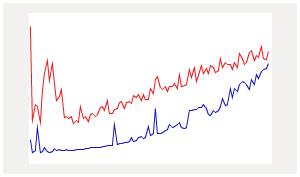
\includegraphics[width=2cm]{graphs/AllInstances}
  \\\hline
  \multicolumn{3}{c}{{\bf Sequence Operations}}\\\hline
  
  Any &
  \lstinputlisting[firstline=2,lastline=3]{transformations/sequence/emftvm/TestAny.atl}
  & 
  	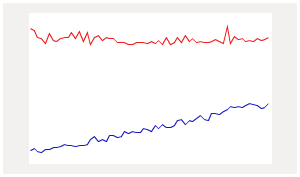
\includegraphics[width=2cm]{graphs/sequence/small/Any}
  \\\hline
  
  Append &
  \lstinputlisting[firstline=2,lastline=3]{transformations/sequence/emftvm/TestAppend.atl}
  & 
  	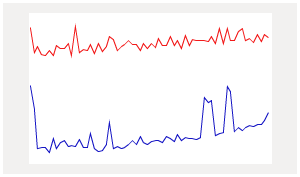
\includegraphics[width=2cm]{graphs/sequence/small/Append}
  \\\hline
  
  At &
  \lstinputlisting[firstline=2,lastline=3]{transformations/sequence/emftvm/TestAt.atl}
  & 
  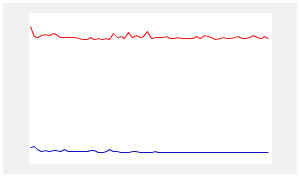
\includegraphics[width=2cm]{graphs/sequence/small/At}
\\\hline

Collect &
\lstinputlisting[firstline=2,lastline=3]{transformations/sequence/emftvm/TestCollect.atl}
&
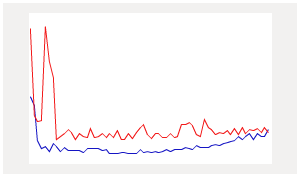
\includegraphics[width=2cm]{graphs/sequence/small/Collect}
\\\hline

EQ &
\lstinputlisting[firstline=2,lastline=3]{transformations/sequence/emftvm/TestEQ.atl}
&
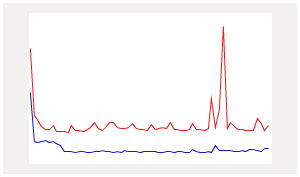
\includegraphics[width=2cm]{graphs/sequence/small/EQ}
\\\hline

Excludes &
\lstinputlisting[firstline=2,lastline=3]{transformations/sequence/emftvm/TestExcludes.atl}
&
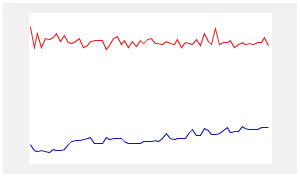
\includegraphics[width=2cm]{graphs/sequence/small/Excludes}
\\\hline

ExcludesAll &
\lstinputlisting[firstline=2,lastline=3]{transformations/sequence/emftvm/TestExcludesAll.atl}
&
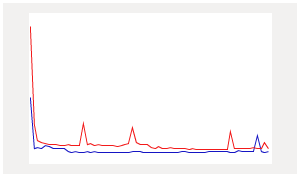
\includegraphics[width=2cm]{graphs/sequence/small/ExcludesAll}
\\\hline

Excluding &
\lstinputlisting[firstline=2,lastline=3]{transformations/sequence/emftvm/TestExcluding.atl}
&
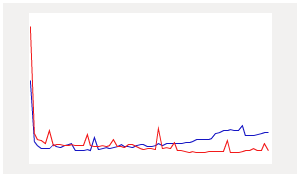
\includegraphics[width=2cm]{graphs/sequence/small/Excluding}
\\\hline

Exists &
\lstinputlisting[firstline=2,lastline=3]{transformations/sequence/emftvm/TestExists.atl}
&
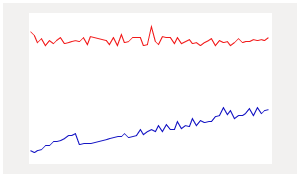
\includegraphics[width=2cm]{graphs/sequence/small/Exists}
\\\hline

First &
\lstinputlisting[firstline=2,lastline=3]{transformations/sequence/emftvm/TestFirst.atl}
&
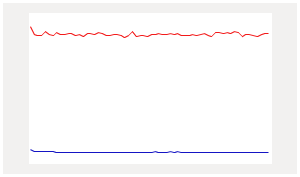
\includegraphics[width=2cm]{graphs/sequence/small/First}
\\\hline

Flatten &
\lstinputlisting[firstline=2,lastline=3]{transformations/sequence/emftvm/TestFlatten.atl}
&
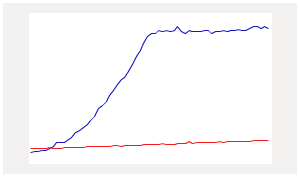
\includegraphics[width=2cm]{graphs/sequence/small/Flatten}
\\\hline

ForAll &
\lstinputlisting[firstline=2,lastline=3]{transformations/sequence/emftvm/TestForAll.atl}
&
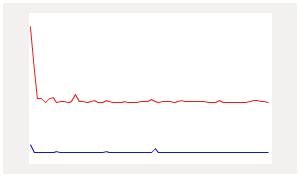
\includegraphics[width=2cm]{graphs/sequence/small/forALL}
\\\hline

Includes &
\lstinputlisting[firstline=2,lastline=3]{transformations/sequence/emftvm/TestIncludes.atl}
&
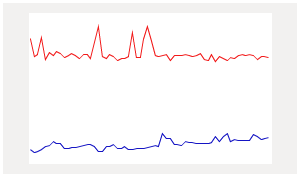
\includegraphics[width=2cm]{graphs/sequence/small/Includes}
\\\hline

IncludesAll &
\lstinputlisting[firstline=2,lastline=3]{transformations/sequence/emftvm/TestIncludesAll.atl}
&
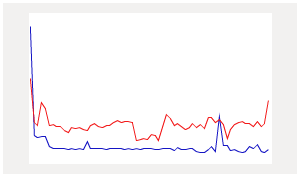
\includegraphics[width=2cm]{graphs/sequence/small/IncludesAll}
\\\hline

Including &
\lstinputlisting[firstline=2,lastline=3]{transformations/sequence/emftvm/TestIncluding.atl}
&
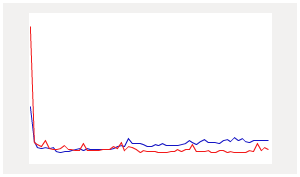
\includegraphics[width=2cm]{graphs/sequence/small/Including}
\\\hline

IndexOf &
\lstinputlisting[firstline=2,lastline=3]{transformations/sequence/emftvm/TestIndexOf.atl}
&
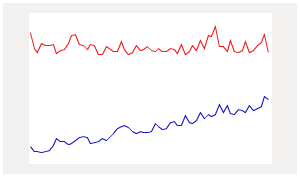
\includegraphics[width=2cm]{graphs/sequence/small/IndexOf}
\\\hline

InsertAt &
\lstinputlisting[firstline=2,lastline=3]{transformations/sequence/emftvm/TestInsertAt.atl}
&
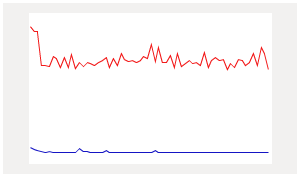
\includegraphics[width=2cm]{graphs/sequence/small/InsertAt}
\\\hline

IsEmpty &
\lstinputlisting[firstline=2,lastline=3]{transformations/sequence/emftvm/TestIsEmpty.atl}
&
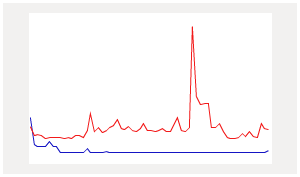
\includegraphics[width=2cm]{graphs/sequence/small/IsEmpty}
\\\hline

IsUnique &
\lstinputlisting[firstline=2,lastline=3]{transformations/sequence/emftvm/TestIsUnique.atl}
&
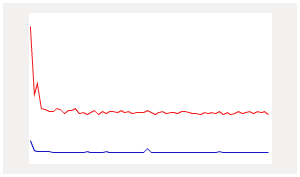
\includegraphics[width=2cm]{graphs/sequence/small/isUnique}
\\\hline

Iterate &
\lstinputlisting[firstline=2,lastline=3]{transformations/sequence/emftvm/TestIterate.atl}
&
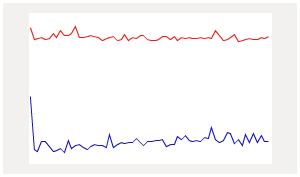
\includegraphics[width=2cm]{graphs/sequence/small/Iterate}
\\\hline

Last &
\lstinputlisting[firstline=2,lastline=3]{transformations/sequence/emftvm/TestLast.atl}
&
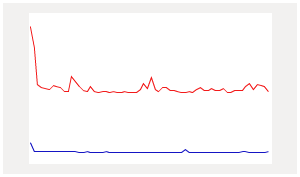
\includegraphics[width=2cm]{graphs/sequence/small/Last}
\\\hline

NotEqual &
\lstinputlisting[firstline=2,lastline=3]{transformations/sequence/emftvm/TestNeq.atl}
&
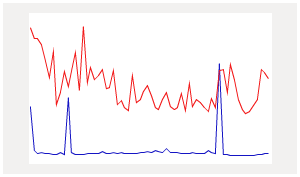
\includegraphics[width=2cm]{graphs/sequence/small/NEQ}
\\\hline

One &
\lstinputlisting[firstline=2,lastline=3]{transformations/sequence/emftvm/TestOne.atl}
&
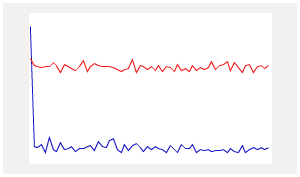
\includegraphics[width=2cm]{graphs/sequence/small/One}
\\\hline

Prepend &
\lstinputlisting[firstline=2,lastline=3]{transformations/sequence/emftvm/TestPrepend.atl}
&
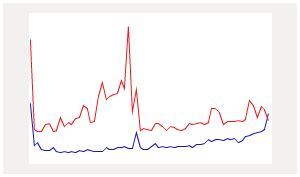
\includegraphics[width=2cm]{graphs/sequence/small/Prepend}
\\\hline

Reject &
\lstinputlisting[firstline=2,lastline=3]{transformations/sequence/emftvm/TestReject.atl}
&
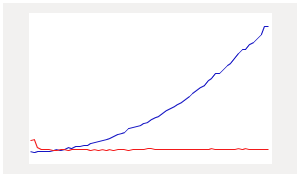
\includegraphics[width=2cm]{graphs/sequence/small/Reject}
\\\hline

Select &
\lstinputlisting[firstline=2,lastline=3]{transformations/sequence/emftvm/TestSelect.atl}
&
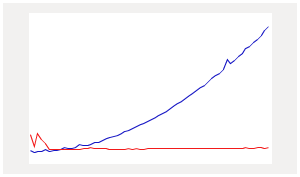
\includegraphics[width=2cm]{graphs/sequence/small/Select}
\\\hline

Size &
\lstinputlisting[firstline=2,lastline=3]{transformations/sequence/emftvm/TestSize.atl}
&
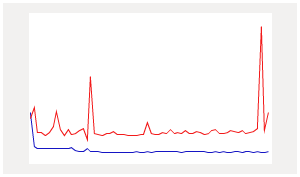
\includegraphics[width=2cm]{graphs/sequence/small/Size}
\\\hline

SortedBy &
\lstinputlisting[firstline=2,lastline=3]{transformations/sequence/emftvm/TestSortedBy.atl}
&
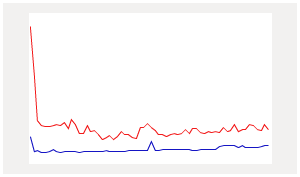
\includegraphics[width=2cm]{graphs/sequence/small/sortedBy}
\\\hline

SubSequence &
\lstinputlisting[firstline=2,lastline=3]{transformations/sequence/emftvm/TestSubsequence.atl}
&
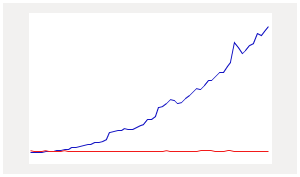
\includegraphics[width=2cm]{graphs/sequence/small/SubSequence}
\\\hline

Sum &
\lstinputlisting[firstline=2,lastline=3]{transformations/sequence/emftvm/TestSum.atl}
&
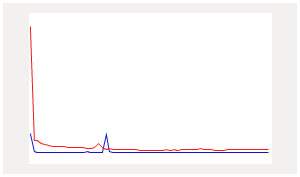
\includegraphics[width=2cm]{graphs/sequence/small/Sum}
\\\hline

Union &
\lstinputlisting[firstline=2,lastline=3]{transformations/sequence/emftvm/TestUnion.atl}
&
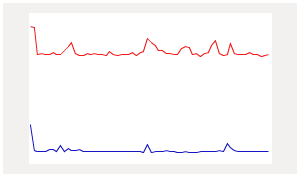
\includegraphics[width=2cm]{graphs/sequence/small/Union}
\\\hline
%%%%%%%%%%%%%%%%%%%%%%%%%%%%%%%%%%%%%%%%%%%%%%%%%%%%%%%%%%%%%%%%%%%%%%%%%%%%%%%%%%%%%%%%%%
%%%%%%%%%%%%%%%%%%%%%%%%%%%%%%%%%%%%%%%%% SET
% %%%%%%%%%%%%%%%%%%%%%%%%%%%%%%%%%%%%%%%%%%%%%%%%%%%%%%%%%%%%%%%%%%%%%%%%%%%%%%%%%%%%
 \multicolumn{3}{c}{{\bf Set Operations}}\\\hline
 
  Any &
  \lstinputlisting[firstline=2,lastline=3]{transformations/set/emftvm/TestAny.atl}
  & 
  	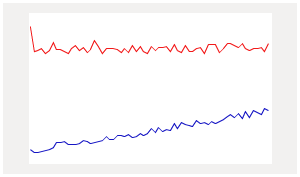
\includegraphics[width=2cm]{graphs/set/small/Any}
  \\\hline
  
  Collect &
\lstinputlisting[firstline=2,lastline=3]{transformations/set/emftvm/TestCollect.atl}
&
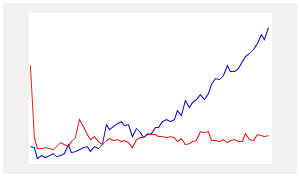
\includegraphics[width=2cm]{graphs/set/small/Collect}
\\\hline

EQ &
\lstinputlisting[firstline=2,lastline=3]{transformations/set/emftvm/TestEQ.atl}
&
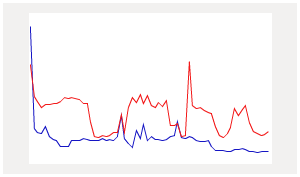
\includegraphics[width=2cm]{graphs/set/small/EQ}
\\\hline

Excludes &
\lstinputlisting[firstline=2,lastline=3]{transformations/set/emftvm/TestExcludes.atl}
&
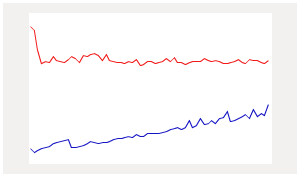
\includegraphics[width=2cm]{graphs/set/small/Excludes}
\\\hline

ExcludesAll &
\lstinputlisting[firstline=2,lastline=3]{transformations/set/emftvm/TestExcludesAll.atl}
&
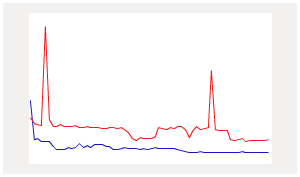
\includegraphics[width=2cm]{graphs/set/small/ExcludesAll}
\\\hline

Excluding &
\lstinputlisting[firstline=2,lastline=3]{transformations/set/emftvm/TestExcluding.atl}
&
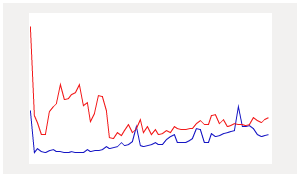
\includegraphics[width=2cm]{graphs/set/small/Excluding}
\\\hline

Exists &
\lstinputlisting[firstline=2,lastline=3]{transformations/set/emftvm/TestExists.atl}
&
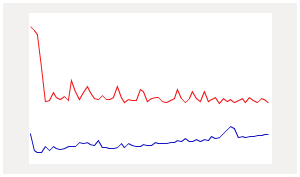
\includegraphics[width=2cm]{graphs/set/small/Exists}
\\\hline

Flatten &
\lstinputlisting[firstline=2,lastline=3]{transformations/set/emftvm/TestFlatten.atl}
&
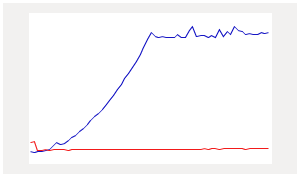
\includegraphics[width=2cm]{graphs/set/small/Flatten}
\\\hline

ForAll &
\lstinputlisting[firstline=2,lastline=3]{transformations/set/emftvm/TestForAll.atl}
&
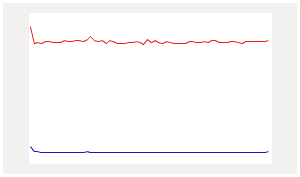
\includegraphics[width=2cm]{graphs/set/small/forALL}
\\\hline

Includes &
\lstinputlisting[firstline=2,lastline=3]{transformations/set/emftvm/TestIncludes.atl}
&
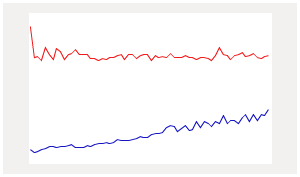
\includegraphics[width=2cm]{graphs/set/small/Includes}
\\\hline

IncludesAll &
\lstinputlisting[firstline=2,lastline=3]{transformations/set/emftvm/TestIncludesAll.atl}
&
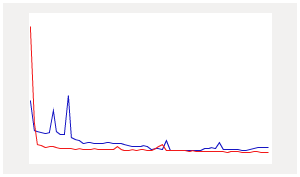
\includegraphics[width=2cm]{graphs/set/small/IncludesAll}
\\\hline

Including &
\lstinputlisting[firstline=2,lastline=3]{transformations/set/emftvm/TestIncluding.atl}
&
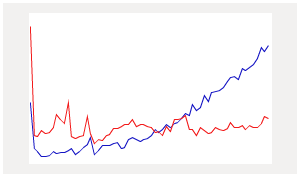
\includegraphics[width=2cm]{graphs/set/small/Including}
\\\hline

Intersection &
\lstinputlisting[firstline=2,lastline=3]{transformations/set/emftvm/TestIntersection.atl}
&
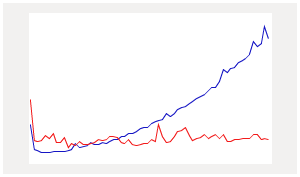
\includegraphics[width=2cm]{graphs/set/small/Intersection}
\\\hline

IsEmpty &
\lstinputlisting[firstline=2,lastline=3]{transformations/set/emftvm/TestIsEmpty.atl}
&
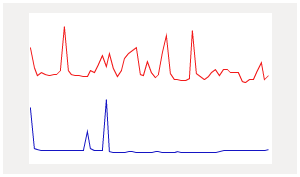
\includegraphics[width=2cm]{graphs/set/small/IsEmpty}
\\\hline

IsUnique &
\lstinputlisting[firstline=2,lastline=3]{transformations/set/emftvm/TestIsUnique.atl}
&
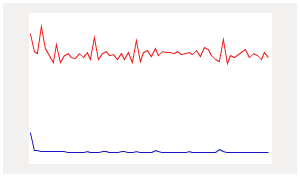
\includegraphics[width=2cm]{graphs/set/small/isUnique}
\\\hline

Iterate &
\lstinputlisting[firstline=2,lastline=3]{transformations/set/emftvm/TestIterate.atl}
&
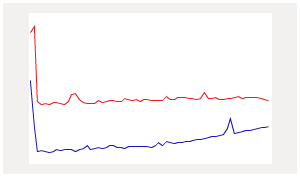
\includegraphics[width=2cm]{graphs/set/small/Iterate}
\\\hline

Minus &
\lstinputlisting[firstline=2,lastline=3]{transformations/set/emftvm/TestMinus.atl}
&
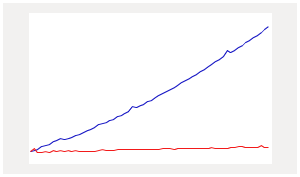
\includegraphics[width=2cm]{graphs/set/small/Minus}
\\\hline

NotEqual &
\lstinputlisting[firstline=2,lastline=3]{transformations/set/emftvm/TestNeq.atl}
&
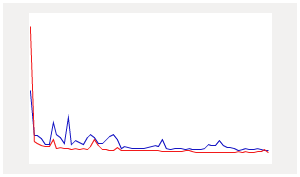
\includegraphics[width=2cm]{graphs/set/small/NEQ}
\\\hline

One &
\lstinputlisting[firstline=2,lastline=3]{transformations/set/emftvm/TestOne.atl}
&
\includegraphics[width=2cm]{graphs/set/small/One}
\\\hline

Reject &
\lstinputlisting[firstline=2,lastline=3]{transformations/set/emftvm/TestReject.atl}
&
\includegraphics[width=2cm]{graphs/set/small/Reject}
\\\hline

Select &
\lstinputlisting[firstline=2,lastline=3]{transformations/set/emftvm/TestSelect.atl}
&
\includegraphics[width=2cm]{graphs/set/small/Select}
\\\hline

Size &
\lstinputlisting[firstline=2,lastline=3]{transformations/set/emftvm/TestSize.atl}
&
\includegraphics[width=2cm]{graphs/set/small/Size}
\\\hline

SortedBy &
\lstinputlisting[firstline=2,lastline=3]{transformations/set/emftvm/TestSortedBy.atl}
&
\includegraphics[width=2cm]{graphs/set/small/sortedBy}
\\\hline

Sum &
\lstinputlisting[firstline=2,lastline=3]{transformations/set/emftvm/TestSum.atl}
&
\includegraphics[width=2cm]{graphs/set/small/Sum}
\\\hline

Symmetric Difference &
\lstinputlisting[firstline=2,lastline=3]{transformations/set/emftvm/TestSymmetricDif.atl}
&
\includegraphics[width=2cm]{graphs/set/small/SymmetricDif}
\\\hline

Union &
\lstinputlisting[firstline=2,lastline=3]{transformations/set/emftvm/TestUnion.atl}
&
\includegraphics[width=2cm]{graphs/set/small/Union}
\\\hline

%%%%%%%%%%%%%%%%%%%%%%%%%%%%%%%%%%%%%%%%%%%%%%%%%%%%%%%%%%%%%%%%%%%%%%%%%%%%%%%%%%%%%%%%%%
%%%%%%%%%%%%%%%%%%%%%%%%%%%%%%%%%%%%%%%%% Bag
% %%%%%%%%%%%%%%%%%%%%%%%%%%%%%%%%%%%%%%%%%%%%%%%%%%%%%%%%%%%%%%%%%%%%%%%%%%%%%%%%%%%%
 \multicolumn{3}{c}{{\bf Bag Operations}}\\\hline
 
 Any &
  \lstinputlisting[firstline=2,lastline=3]{transformations/bag/emftvm/TestAny.atl}
  & 
  	\includegraphics[width=2cm]{graphs/bag/small/Any}
  \\\hline
  
  Collect &
\lstinputlisting[firstline=2,lastline=3]{transformations/bag/emftvm/TestCollect.atl}
&
\includegraphics[width=2cm]{graphs/bag/small/Collect}
\\\hline

EQ &
\lstinputlisting[firstline=2,lastline=3]{transformations/bag/emftvm/TestEQ.atl}
&
\includegraphics[width=2cm]{graphs/bag/small/EQ}
\\\hline

Excludes &
\lstinputlisting[firstline=2,lastline=3]{transformations/bag/emftvm/TestExcludes.atl}
&
\includegraphics[width=2cm]{graphs/bag/small/Excludes}
\\\hline

ExcludesAll &
\lstinputlisting[firstline=2,lastline=3]{transformations/bag/emftvm/TestExcludesAll.atl}
&
\includegraphics[width=2cm]{graphs/bag/small/ExcludesAll}
\\\hline

Excluding &
\lstinputlisting[firstline=2,lastline=3]{transformations/bag/emftvm/TestExcluding.atl}
&
\includegraphics[width=2cm]{graphs/bag/small/Excluding}
\\\hline

Exists &
\lstinputlisting[firstline=2,lastline=3]{transformations/bag/emftvm/TestExists.atl}
&
\includegraphics[width=2cm]{graphs/bag/small/Exists}
\\\hline

Flatten &
\lstinputlisting[firstline=2,lastline=3]{transformations/bag/emftvm/TestFlatten.atl}
&
\includegraphics[width=2cm]{graphs/bag/small/Flatten}
\\\hline

ForAll &
\lstinputlisting[firstline=2,lastline=3]{transformations/bag/emftvm/TestForAll.atl}
&
\includegraphics[width=2cm]{graphs/bag/small/forALL}
\\\hline

Includes &
\lstinputlisting[firstline=2,lastline=3]{transformations/bag/emftvm/TestIncludes.atl}
&
\includegraphics[width=2cm]{graphs/bag/small/Includes}
\\\hline

IncludesAll &
\lstinputlisting[firstline=2,lastline=3]{transformations/bag/emftvm/TestIncludesAll.atl}
&
\includegraphics[width=2cm]{graphs/bag/small/IncludesAll}
\\\hline

Including &
\lstinputlisting[firstline=2,lastline=3]{transformations/bag/emftvm/TestIncluding.atl}
&
\includegraphics[width=2cm]{graphs/bag/small/Including}
\\\hline

IsEmpty &
\lstinputlisting[firstline=2,lastline=3]{transformations/bag/emftvm/TestIsEmpty.atl}
&
\includegraphics[width=2cm]{graphs/bag/small/IsEmpty}
\\\hline

IsUnique &
\lstinputlisting[firstline=2,lastline=3]{transformations/bag/emftvm/TestIsUnique.atl}
&
\includegraphics[width=2cm]{graphs/bag/small/isUnique}
\\\hline

Iterate &
\lstinputlisting[firstline=2,lastline=3]{transformations/bag/emftvm/TestIterate.atl}
&
\includegraphics[width=2cm]{graphs/bag/small/Iterate}
\\\hline

NotEqual &
\lstinputlisting[firstline=2,lastline=3]{transformations/bag/emftvm/TestNeq.atl}
&
\includegraphics[width=2cm]{graphs/bag/small/NEQ}
\\\hline

One &
\lstinputlisting[firstline=2,lastline=3]{transformations/bag/emftvm/TestOne.atl}
&
\includegraphics[width=2cm]{graphs/bag/small/One}
\\\hline

Reject &
\lstinputlisting[firstline=2,lastline=3]{transformations/bag/emftvm/TestReject.atl}
&
\includegraphics[width=2cm]{graphs/bag/small/Reject}
\\\hline

Select &
\lstinputlisting[firstline=2,lastline=3]{transformations/bag/emftvm/TestSelect.atl}
&
\includegraphics[width=2cm]{graphs/bag/small/Select}
\\\hline

Size &
\lstinputlisting[firstline=2,lastline=3]{transformations/bag/emftvm/TestSize.atl}
&
\includegraphics[width=2cm]{graphs/bag/small/Size}
\\\hline

SortedBy &
\lstinputlisting[firstline=2,lastline=3]{transformations/bag/emftvm/TestSortedBy.atl}
&
\includegraphics[width=2cm]{graphs/bag/small/sortedBy}
\\\hline

Sum &
\lstinputlisting[firstline=2,lastline=3]{transformations/bag/emftvm/TestSum.atl}
&
\includegraphics[width=2cm]{graphs/bag/small/Sum}
\\\hline
 
 %%%%%%%%%%%%%%%%%%%%%%%%%%%%%%%%%%%%%%%%%%%%%%%%%%%%%%%%%%%%%%%%%%%%%%%%%%%%%%%%%%%%%%%%%%
%%%%%%%%%%%%%%%%%%%%%%%%%%%%%%%%%%%%%%%%% OrderedSet
% %%%%%%%%%%%%%%%%%%%%%%%%%%%%%%%%%%%%%%%%%%%%%%%%%%%%%%%%%%%%%%%%%%%%%%%%%%%%%%%%%%%%
 \multicolumn{3}{c}{{\bf OrderedSet Operations}}\\\hline
 
 Any &
  \lstinputlisting[firstline=2,lastline=3]{transformations/orderedset/emftvm/TestAny.atl}
  & 
  	\includegraphics[width=2cm]{graphs/orderedset/small/Any}
  \\\hline
  
  Append &
  \lstinputlisting[firstline=2,lastline=3]{transformations/orderedset/emftvm/TestAppend.atl}
  & 
  	\includegraphics[width=2cm]{graphs/orderedset/small/Append}
  \\\hline
  
  At &
  \lstinputlisting[firstline=2,lastline=3]{transformations/orderedset/emftvm/TestAt.atl}
  & 
  \includegraphics[width=2cm]{graphs/orderedset/small/At}
\\\hline

Collect &
\lstinputlisting[firstline=2,lastline=3]{transformations/orderedset/emftvm/TestCollect.atl}
&
\includegraphics[width=2cm]{graphs/orderedset/small/Collect}
\\\hline

EQ &
\lstinputlisting[firstline=2,lastline=3]{transformations/orderedset/emftvm/TestEQ.atl}
&
\includegraphics[width=2cm]{graphs/orderedset/small/EQ}
\\\hline

Excludes &
\lstinputlisting[firstline=2,lastline=3]{transformations/orderedset/emftvm/TestExcludes.atl}
&
\includegraphics[width=2cm]{graphs/orderedset/small/Excludes}
\\\hline

ExcludesAll &
\lstinputlisting[firstline=2,lastline=3]{transformations/orderedset/emftvm/TestExcludesAll.atl}
&
\includegraphics[width=2cm]{graphs/orderedset/small/ExcludesAll}
\\\hline

Excluding &
\lstinputlisting[firstline=2,lastline=3]{transformations/orderedset/emftvm/TestExcluding.atl}
&
\includegraphics[width=2cm]{graphs/orderedset/small/Excluding}
\\\hline

Exists &
\lstinputlisting[firstline=2,lastline=3]{transformations/orderedset/emftvm/TestExists.atl}
&
\includegraphics[width=2cm]{graphs/orderedset/small/Exists}
\\\hline

First &
\lstinputlisting[firstline=2,lastline=3]{transformations/orderedset/emftvm/TestFirst.atl}
&
\includegraphics[width=2cm]{graphs/orderedset/small/First}
\\\hline

Flatten &
\lstinputlisting[firstline=2,lastline=3]{transformations/orderedset/emftvm/TestFlatten.atl}
&
\includegraphics[width=2cm]{graphs/orderedset/small/Flatten}
\\\hline

ForAll &
\lstinputlisting[firstline=2,lastline=3]{transformations/orderedset/emftvm/TestForAll.atl}
&
\includegraphics[width=2cm]{graphs/orderedset/small/forALL}
\\\hline

Includes &
\lstinputlisting[firstline=2,lastline=3]{transformations/orderedset/emftvm/TestIncludes.atl}
&
\includegraphics[width=2cm]{graphs/orderedset/small/Includes}
\\\hline

IncludesAll &
\lstinputlisting[firstline=2,lastline=3]{transformations/orderedset/emftvm/TestIncludesAll.atl}
&
\includegraphics[width=2cm]{graphs/orderedset/small/IncludesAll}
\\\hline

Including &
\lstinputlisting[firstline=2,lastline=3]{transformations/orderedset/emftvm/TestIncluding.atl}
&
\includegraphics[width=2cm]{graphs/orderedset/small/Including}
\\\hline

IndexOf &
\lstinputlisting[firstline=2,lastline=3]{transformations/orderedset/emftvm/TestIndexOf.atl}
&
\includegraphics[width=2cm]{graphs/orderedset/small/IndexOf}
\\\hline

InsertAt &
\lstinputlisting[firstline=2,lastline=3]{transformations/orderedset/emftvm/TestInsertAt.atl}
&
\includegraphics[width=2cm]{graphs/orderedset/small/InsertAt}
\\\hline

IsEmpty &
\lstinputlisting[firstline=2,lastline=3]{transformations/orderedset/emftvm/TestIsEmpty.atl}
&
\includegraphics[width=2cm]{graphs/orderedset/small/IsEmpty}
\\\hline

IsUnique &
\lstinputlisting[firstline=2,lastline=3]{transformations/orderedset/emftvm/TestIsUnique.atl}
&
\includegraphics[width=2cm]{graphs/orderedset/small/isUnique}
\\\hline

Iterate &
\lstinputlisting[firstline=2,lastline=3]{transformations/orderedset/emftvm/TestIterate.atl}
&
\includegraphics[width=2cm]{graphs/orderedset/small/Iterate}
\\\hline

Last &
\lstinputlisting[firstline=2,lastline=3]{transformations/orderedset/emftvm/TestLast.atl}
&
\includegraphics[width=2cm]{graphs/orderedset/small/Last}
\\\hline

NotEqual &
\lstinputlisting[firstline=2,lastline=3]{transformations/orderedset/emftvm/TestNeq.atl}
&
\includegraphics[width=2cm]{graphs/orderedset/small/NEQ}
\\\hline

One &
\lstinputlisting[firstline=2,lastline=3]{transformations/orderedset/emftvm/TestOne.atl}
&
\includegraphics[width=2cm]{graphs/orderedset/small/One}
\\\hline

Prepend &
\lstinputlisting[firstline=2,lastline=3]{transformations/orderedset/emftvm/TestPrepend.atl}
&
\includegraphics[width=2cm]{graphs/orderedset/small/Prepend}
\\\hline

Reject &
\lstinputlisting[firstline=2,lastline=3]{transformations/orderedset/emftvm/TestReject.atl}
&
\includegraphics[width=2cm]{graphs/orderedset/small/Reject}
\\\hline

Select &
\lstinputlisting[firstline=2,lastline=3]{transformations/orderedset/emftvm/TestSelect.atl}
&
\includegraphics[width=2cm]{graphs/orderedset/small/Select}
\\\hline

Size &
\lstinputlisting[firstline=2,lastline=3]{transformations/orderedset/emftvm/TestSize.atl}
&
\includegraphics[width=2cm]{graphs/orderedset/small/Size}
\\\hline

SortedBy &
\lstinputlisting[firstline=2,lastline=3]{transformations/orderedset/emftvm/TestSortedBy.atl}
&
\includegraphics[width=2cm]{graphs/orderedset/small/sortedBy}
\\\hline

Suborderedset &
\lstinputlisting[firstline=2,lastline=3]{transformations/orderedset/emftvm/TestSubOrderedSet.atl}
&
\includegraphics[width=2cm]{graphs/orderedset/small/Suborderedset}
\\\hline

Sum &
\lstinputlisting[firstline=2,lastline=3]{transformations/orderedset/emftvm/TestSum.atl}
&
\includegraphics[width=2cm]{graphs/orderedset/small/Sum}
\\\hline

Union &
\lstinputlisting[firstline=2,lastline=3]{transformations/orderedset/emftvm/TestUnion.atl}
&
\includegraphics[width=2cm]{graphs/orderedset/small/Union}
\\\hline
  
%\end{tabular}
%\end{center}
\caption{Evaluation Results }
\label{tab:resultsFull}
\end{longtable}


